\chapter{Implementation} \label{chap:impl}

This chapter provides a detailed description of the implemented system. In Section~\ref{sec:impl-GM}, the Geometric Monitoring method implementation is described, along with the necessary simplyfing assumptions to aid experimentation. Following that, in Section~\ref{sec:impl-distNodeMatch} an algorithm for node matching is proposed, inspired by the violation recovery method found in~\cite{Keren2014GMHetStreams}. In Section~\ref{sec:impl-heuristic}, the heuristic based balancing method for local violation resolution is presented, along with the necessary data stream tracking scheme. Finally, the main implementation challenges are discussed.

\section{Geometric Monitoring Implementation} \label{sec:impl-GM}

The initial Geometric Monitoring method~\cite{Sharfman2006GM}, which is described in detail in Section~\ref{sec:theorBack-GM}, provides two algorithms for threshold monitoring of distributed data streams. These algorithms operate on different network structures and implement a somewhat different handling of threshold violations.

The decentralized algorithm operates on a coordinator-less enviroment, where nodes are allowed to communicate with each other, whereas the coordinator-based algorithm has a Star network topology, where the coordinator node is the central node (the \emph{hub}) and the Monitoring nodes recide on the edges of the network.
The algorithm operating on the decentralized setting does not provide a balancing process for local violation resolution. On the other hand, the coordinator based algorithm implements a violation resolution operation every time a local violation occurs, which aims to minimize the communication overhead induced by false violation reports. 

Our focus is centered towards a simplified \textbf{coordinator-based algorithm} (Algorithm~\ref{algo:GM-coordBased}), described in Section~\ref{sec:theorBack-GM}, as it provides a framework for the heuristic balancing process, as well as the node matching operation presented in detail in Sections~\ref{sec:impl-heuristic} and~\ref{sec:impl-distNodeMatch} respectively.

To aid method formulation and experimentation, the following simplifying assumptions have been made regarding the coordinator-based algorithm:
\begin{itemize}
\item Communication between nodes is considered instantaneous. There is no delay when passing messages through the network. The problem of message handling in a real-world Geometric Monitoring method implementation, where message delays are induced by the underlying network, has been studied in detail in~\cite{Babis2013SimulatorStreams}.

\item Communication between nodes is considered loss-less and reliable. In case network reliability can not be guaranteed appropriate methods should be considered.

\item The system operates in an iterative fashion, as described in Algorithm~\ref{algo:singleHandlingNetwork}. This simplification of the real-time distributed monitoring process to an iterative process provides a more manageable setting for experimentation without distorting the results of the proposed methods, which can be applied directly to the original real-time distributed setting.

\item The system pauses at each violation, until the violation is resolved. During violation resolution Monitoring nodes do not receive updates from their respective data streams.

\item The Coordinator node does not participate in the monitoring operation. The Coordinator node does not receive updates from a data stream, it only receives messages from the Monitoring nodes in case of threshold violation.

\end{itemize}

%TODO: mention training and testing dataset?
%TODO: implementation specifics, ball computation (i.e. optimization)?

%%%%%%%%%%%%%%%%%%%%%%%%%%%%%%%%%%%%%%%% single handling network algo %%%%%%%%%%%%%%%%%%%%%%%%%%%%%%%%%%%%%%%%%%%
\begin{algorithm}[H]
\setstretch{1.30}

\KwData{$monitoringNodes$: a list of Monitoring nodes,~$coordinator$: the Coordinator node}

\SetAlgoLined
\Begin{
 initialization\;
 	\Repeat{$globalViolation$}{
		\ForEach{$node \in\ monitoringNodes$}{
			$node.DataVectorUpdate()$\;
			$node.ComputeDriftVector()$\;
		}
		\ForEach{$node \in\ monitoringNodes$}{
			$node.CheckForViolation()$\;
			\If{$localViolation$}{
				$node.Report()$\;
				$coordinator.Balance()$\;
			}
		}
	}
}
\caption{Iterative network operation \label{algo:singleHandlingNetwork}} 
\end{algorithm}
%%%%%%%%%%%%%%%%%%%%%%%%%%%%%%%%%%%%%%%%%%%%%%%%%%%%%%%%%%%%%%%%%%%%%%%%%%%%%%%%%%%%%%%%%%%%%%%%%%%%%%%%%%%%%%%

\section{Distance Based Node Matching} \label{sec:impl-distNodeMatch}
%TODO: check my notes for things to add

The balancing method of the coordinator-based algorithm, as described in Section~\ref{sec:theorBack-GM}~\cite{Sharfman2006GM, Sharfman2008ShapeSensGM}, aims at resolving local violations that do not result in a global violation (\emph{false alarms}) by balancing the violating node's drift vector with the respective vectors of randomly chosen nodes. Consider the violating node $n_i$ with weight $w_i=1$, so that the bounding ball $B(\vec{e}(t), \vec{u_i}(t))$ is not monochromatic, and the randomly requested node $n_j$ with weight $w_j=1$, so that the newly formed bounding ball is $B(\vec{e}(t), \frac{\vec{u_i}(t)+\vec{u_j}(t)}{2})$, where $\vec{e}(t)$ the estimate vector at time $t$ and $\vec{u_i}(t)$, $\vec{u_j}(t)$ the drift vectors of nodes $n_i$, $n_j$ at time $t$, respectively. If the resulting bounding ball is monochromatic the violation is resolved, otherwise another node is randomly requested for balancing.

As observed in~\cite{Keren2014GMHetStreams}, the original balancing method's node choosing scheme can be inefficient, so a more efficient and deterministic approach should be adopted. Optimal pairing of nodes and the construction of a hierarchical structure (Figure~\ref{fig:nodePairHierarchy}) reduces the communication overhead of false alarms, with the vast majority of violation resolutions requiring only the assigned node pair to be successful. The criterion by which nodes are paired attempts to maximize the probability of a successful balance by maximizing \textit{``the percentage of pairs of data vectors from both nodes whose sum is in the Minkowski sum of the nodes' safe-zones''}~\cite{Keren2014GMHetStreams}, or, in this case, whose resulting bounding ball is monochromatic.

Here, the same node pairing scheme is followed, but with a different, distance based, criterion for grouping nodes into disjoint pairs and creating the hierarchical structure depicted in Figure~\ref{fig:nodePairHierarchy}. The method proceeds as follows (Algorithm~\ref{algo:nodeMatching}):
\begin{enumerate}
\item Monitoring nodes are visualized as the nodes of a complete graph $G=(V,E)$, where $V=\{n_1, n_2, ... , n_k\}$ vertex set consists of the initial Monitoring nodes (\emph{``Type-1 nodes''}) and $E=\{(n_i, n_j)\ \forall i,j \in [1, ..., k], i \neq j\}$ edge set contains an edge for every pair of vertices.
\item Weights are assigned to all edges $E$. The weight of each edge is defined as the cumulative distance of the value of the monitoring function on the mean of each pair of data vectors from the value of the monitoring function on the \emph{global} mean of all Monitoring nodes' data vectors, plus the cumulative distance of each pair of data vectors:
\begin{equation}
w_{i,j}=
\sum_{t=t_0}^{t_{end}}{[(f(\vec{v}_{global}(t))-f(\frac{\vec{v_i}(t)+\vec{v_j}(t)}{2}))+(|\vec{v_i}(t)-\vec{v_j}(t)|)]}
\label{form:distanceMatchingWeights}
\end{equation}
, where $\vec{v_i}(t)$ the data update of node $n_i$ at time $t$, $\vec{v}_{global}(t)$ the global mean of all Monitoring nodes at time $t$ and $f(\cdot)$ the monitoring function.

\item Maximum weighted matching is performed on the resulting graph, so that nodes are partitioned into disjoined sets $M_i$, $|M_i|=2\ \forall i \in [1, ..., \frac{k}{2}]$. 

\item Each set $M_i, i \in [1, ..., \frac{k}{2}]$ is considered a single node, so that a new complete graph $G'=(V', E')$ is created, where $V'=\{M_1, ..., M_{\frac{k}{2}}\}$ (\emph{``Type-2 nodes''}) the new vertex set and $E'=\{(M_i, M_j)\ \forall i,j \in [1, ..., \frac{k}{2}]\}$ the new edge set. Weights are assigned to the new edges and the process repeats until the resulting graph contains only a single vertex (\emph{``Type-k node''}), which incorporates all the initial Monitoring nodes.

\item Vertices not matched with any other vertex during the matching process are ignored in future iterations. During the balancing process such unmatched vertices are handled by the traditional random selection balancing algorithm found in~\cite{Sharfman2006GM}(also, Section~\ref{sec:impl-GM}). 
\end{enumerate} 
~
%%%%%%%%%%%%%%%%%%%%%%%%%%%%%%%%%%%% hierarchy figure %%%%%%%%%%%%%%%%%%%%%%%%%%%%%%%%%%%%
\begin{figure}
\centering
\includegraphics[trim=0 9cm 0 0]{img/NodeMatchingHierarchy.tex}
\caption{Hierarchical pairing scheme example  for node set $\{n_1, n_2, n_3, n_4, n_5, n_6, n_7, n_8\}$.} 
\label{fig:nodePairHierarchy}
\end{figure}
%%%%%%%%%%%%%%%%%%%%%%%%%%%%%%%%%%%%%%%%%%%%%%%%%%%%%%%%%%%%%%%%%%%%%%%%%%%%%%%%%%%%%%%%%%%

%%%%%%%%%%%%%%%%%%%%%%%%%%%%%%%%%%%% node matching algo %%%%%%%%%%%%%%%%%%%%%%%%%%%%%%%%%%%
\begin{algorithm}[H]
\SetAlgoLined
\setstretch{1.30}
\SetKwFunction{DistancePairer}{DistancePairer}
\SetKwProg{Fn}{Function}{}{end}
\Fn{\DistancePairer{$nodes$,$i$}}{
	\KwData{$nodes=[(n_1, [\vec{v_1}(t_0), ... , \vec{v_1}(t_{end})]), ... , (n_k, [\vec{v_k}(t_0), ... , \vec{v_k}(t_{end})])]$: list of nodes with their respective data vectors, $i$: pair type, initial=1} 
	\KwResult{$nodeHierarchy$: dictionary of \emph{Type-k} pairs}

	\If(\tcp*[f]{recursion stoping condition}){$length(nodes)=1$}{
		\Return{$nodeHierarchy$}\;
	}
	$g=CreateCompleteGraph(nodes)$\tcp*[r]{complete graph with $nodes$ as vertices} 
	\ForEach(\tcp*[f]{assign weights to edges}){$(n_i, n_j)\in g.Edges()$}{
		$w_{i,j}=
		\sum_{t=t_0}^{t_{end}}{[(f(\vec{v}_{global}(t))-f(\frac{\vec{v_i}(t)+\vec{v_j}(t)}{2}))+(|\vec{v_i}(t)-\vec{v_j}(t)|)]}$\;
		$g.edge(n_i, n_j).weight=w_{i,j}$\;
	}
	$nodeHierarchy(\text{Type-i})=g.maximalWeightMatching()$\tcp*[r]{node pairs of \emph{Type-}$i$}
	\DistancePairer{$nodeHierarchy(\text{Type-i}),i*2$}\;
}
\caption{Recursively create Monitoring node pairs and hierarchy \label{algo:nodeMatching}} 
\end{algorithm}
%%%%%%%%%%%%%%%%%%%%%%%%%%%%%%%%%%%%%%%%%%%%%%%%%%%%%%%%%%%%%%%%%%%%%%%%%%%%%%%%%%%%%%%%%%%
~
%%%%%%%%%%%%%%%%%%%%%%%%%%%%%%%%%%%% distance figure %%%%%%%%%%%%%%%%%%%%%%%%%%%%%%%%%%%%    
\begin{figure}
        \centering
		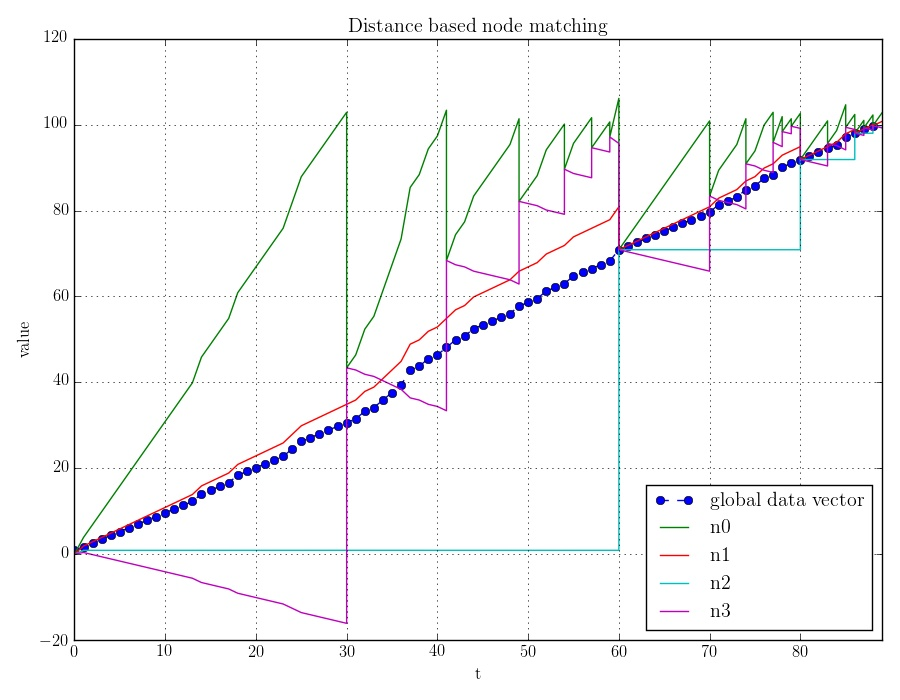
\includegraphics[scale=0.33]{img/distoptpair_example_full.jpeg}
        \caption{The drift vectors during Geometric Monitoring operation until a Global Violation. Distance based node matching is used on 4 nodes ($\{n_0, n_1, n_2, n_3\}$), with 1-dimensional data vectors, threshold $T=100$ and $f(x)=x$ as the monitoring function. The \emph{Type-2} node pairs are $\{n_0, n_3\}$ and $\{n_1, n_2\}$.}\label{fig:distoptpair}
\end{figure}
\begin{figure}
        \centering
		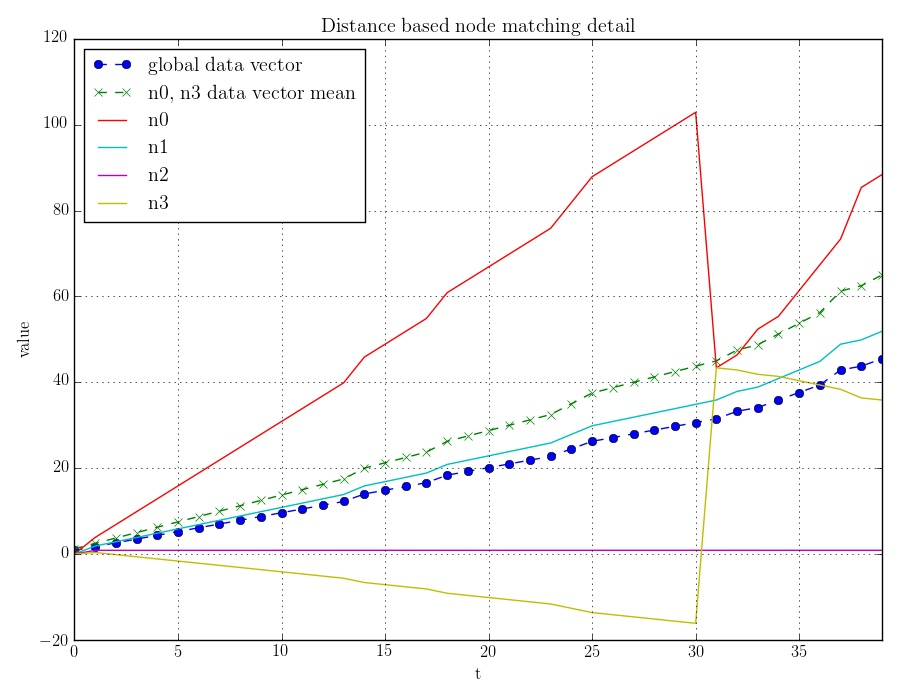
\includegraphics[scale=0.23]{img/distoptpair_example_detail.png}
        \caption{Detailed depiction of the Geometric Monitoring operation of Figure~\ref{fig:distoptpair}. Distance based node matching operating on 4 nodes ($\{n_0, n_1, n_2, n_3\}$), with 1-dimensional data vectors, threshold $T=100$ and $f(x)=x$ as the monitoring function. Distance $d_1$ denotes the distance of the data vector mean of the paired nodes $n_0$ and $n_3$ from the global mean (\emph{global data vector}) at $t=25$, whereas distance $d_2$ denotes the inbetween distance of data vectors $\vec{v_0}(t)$ and $\vec{v_3}(t)$ of the node pair at time $t=25$ (before a Local Violation occures, where $\vec{e}=0$ and $\vec{u_i}(t)=\vec{v_i}(t)\ \forall\ i\in[0,1,2,3], t<30$). Both distances are taking part in the edge weighting process, according to Equation~\ref{form:distanceMatchingWeights}.} \label{fig:distoptpairdetailed}
\end{figure}%

%%%%%%%%%%%%%%%%%%%%%%%%%%%%%%%%%%%%%%%%%%%%%%%%%%%%%%%%%%%%%%%%%%%%%%%%%%%%%%%%%%%%%%%%%%%

The incentive behind the distance based node pairing scheme comes from the need to track the global data vector as closely as possible, with only a subset of the total node population's data vectors at each balancing attempt. By considering the distance of the mean of a pair of data vectors from the global data vector (distance $d_1$ in Figure~\ref{fig:distoptpairdetailed}) the \emph{``quality''} and \emph{``accuracy''} of the tracking ability of each pair is evaluated. Additionally, by taking into account the inbetween distance of data vectors of each node pair (distance $d_2$ in Figure~\ref{fig:distoptpairdetailed}), pairs from the limits of the data vector velocity spectrum that manage to \emph{``cancel each other out''} more effectively are encouraged.
\newpage
\section{Heuristic Balancing} \label{sec:impl-heuristic}
%TODO: check notes for additional stuff to add
balancing process in original gm(1 paragraph)

why the original method looses points\\
mention estimate vector moving and custom shapes as attempts to optimize balance vector computation

our approach: optimaly position new drift vectors to maxinize the time until a local violation.\\
use simple velocity and acceleration estimations of drift vectors to enhance results.

the heuristic formula and explain

images of optimal positions in 2-d (3-d?)

sketch of convex hull and balls and otimal positions vs traditional positioning (2-d)

analyze the method (bilevel multiobjective optimization), write the formulas of optimization (stackoverflow style)\\
mention solvers used 

algorithm

%%%%%%%%%%%%%%%%%%%%%%%%%%%%%%%%%%%% balancing figure %%%%%%%%%%%%%%%%%%%%%%%%%%%%%%%%%%%%
\begin{figure*}[t!]
\centering
\begin{subfigure}[t]{0.45\textwidth}
\centering
\includegraphics[scale=0.45]{img/classic_balancing.tex}
\caption{Hierarchical pairing scheme example  for node set $\{n_1, n_2, n_3, n_4, n_5, n_6, n_7, n_8\}$.} 
%\label{fig:nodePairHierarchy}
\end{subfigure}
\begin{subfigure}[t]{0.45\textwidth}
\centering
\includegraphics[scale=0.45]{img/heuristic_balancing.tex}
\caption{Hierarchical pairing scheme example  for node set $\{n_1, n_2, n_3, n_4, n_5, n_6, n_7, n_8\}$.} 
%\label{fig:nodePairHierarchy}
\end{subfigure}
\caption{Balancing schemes}
\end{figure*}
%%%%%%%%%%%%%%%%%%%%%%%%%%%%%%%%%%%%%%%%%%%%%%%%%%%%%%%%%%%%%%%%%%%%%%%%%%%%%%%%%%%%%%%%%%%

\subsection{Smoothing, Velocity and Acceleration Estimation via Savitzky-Golay} \label{subsec:impl-heuristic-vel}

why S-G:
smoothing and derivation at the same time\\
precomputed coefficients (real time)\\
easy implementation\\
customizable(window and order)\\

S-G implementation and algorithm\\

Example images of same data smoothed, velocity and acceleration (3 figures or all in one?)

\section{Implementation Challenges} \label{sec:impl-implChallenges}

training data\\
can be overcome, worst case scenario our algorithm operates just like the original GM

complexity of optimization (i.e. optimal point location)

complexity of optimization (i.e. node matching)